%!TEX root=main.tex
\section{ClickNP Elements}
\label{clicknp:sec:elements}

In this section we show LOC (Line Of Code) (excluding host program) and resource utilization of some common elements under reasonable parameter settings.

All elements shown in this section can process 40 Gbps line rate for all Ethernet packet sizes under 190 MHz clock rate, i.e. one cycle per iteration for elements processing packet flits, and up to 3 cycles per iteration for elements processing metadata only.

\subsection{Basic Connectors}

\begin{table}[h!]
	\centering
	\label{clicknp:tab:Basic Connectors}
	\begin{tabular}{l|r|r|r}
		Element & LOC & Logic & Memory \\
		\hline
		Tee	&  & \%  & 0\% \\
		Mux	&  & \% & 0\% \\
		Demux & & \% & 0\% \\
		FlitMux & & \% & 0\% \\
		FlitDemux & & \% & 0\% \\
	\end{tabular}
\end{table}


\subsection{Programmable Header Parser}

Packet parser is an important part of network processor, whose complexity comes from tunneling protocols and diversity of protocols in each layer.

The uncertainty of outer layers introduce non-constant header offset in the packet. For example, an Ethernet packet without VLAN has IP header offset 14, an Ethernet packet with VLAN has IP header offset 18. Simply using a variable as index to packet byte array is very ineffective in OpenCL. An array with one or more variable index access will be implemented as block SRAM in FPGA, which only support one read operation per cycle. In order to parse the packet header (which includes many array accesses) in one cycle, we need to implement the packet buffer as register in FPGA, which requires all accesses to the packet buffer array to have constant index.

%If we create an element for each packet header, then each element needs to shift the packet payload in order to ``peel off'' the parsed header. The first drawback is that each element introduces some overhead in logic utilization. Since there are multiple leaf elements representing the innermost header to parse, and different elements have different latencies, output packets at the final mux will be out-of-order. The reordering buffer would take considerable local memory. Furthermore, in the case of network virtualization and tunneled protocols, there will be a loop of elements that each tunneled packet would travel twice, which lowers throughput of packet parser.

To implement a packet parser with all packet buffer offsets to be constant, without shifting packet payload after each header is parsed, we need to enumerate all possible parsing paths (e.g. Ethernet $\rightarrow$ IP, Ethernet $\rightarrow$ VLAN $\rightarrow$ IP), duplicate parser code for each path and calculate offset for each access to packet buffer. Doing such work manually is frustrating and error-prone, therefore ClickNP provides a general \textit{.state\_machine} abstraction, which can generate a decision tree composed of all possible state migration paths and calculate all packet buffer offsets at compilation time.

\begin{lstlisting}
.state_machine {
    constexpr offset = 0;
    .parser_define MAX_STATE_REPEAT 2;
    begin {
        constexpr offset += 12;
        ushort next_proto = *(ushort *) &input[offset];
        constexpr offset += 2;
        if (next_proto == PROTO_VLAN)
            .goto_state VLAN;
        else if (next_proto == PROTO_IPv4)
            .goto_state IPv4;
        else
            .goto_state end;
    }
    VLAN {
        if (!meta.vlan)
            meta.vlan = *(ushort *) input[offset];
        ushort next_proto = *(ushort *) &input[offset + 2];
        constexpr offset += 4;
        if (next_proto == 0x8100)
            .goto_state VLAN;
        else if (next_proto == 0x0800)
            .goto_state IPv4;
        else
            .goto_state end;
    }
    IPv4 {
        .if (STATE_REPEAT == 1) {
            meta.src_ip = *(uint *) &input[offset + 12];
            meta.dst_ip = *(uint *) &input[offset + 16];
        } .else {
            meta.inner_src_ip = *(uint *) &input[offset + 12];
            meta.inner_dst_ip = *(uint *) &input[offset + 16];
        }
        ushort next_proto = input[offset + 9];
        constexpr offset += 20;
        if (next_proto == 94)
            .goto_state IPv4; // IP-in-IP
        else if (next_proto == 97)
            .goto_state begin; // ETHERIP
        else
            .goto_state end;
    }
}
\end{lstlisting}


\begin{figure}[!t]
	\centering
	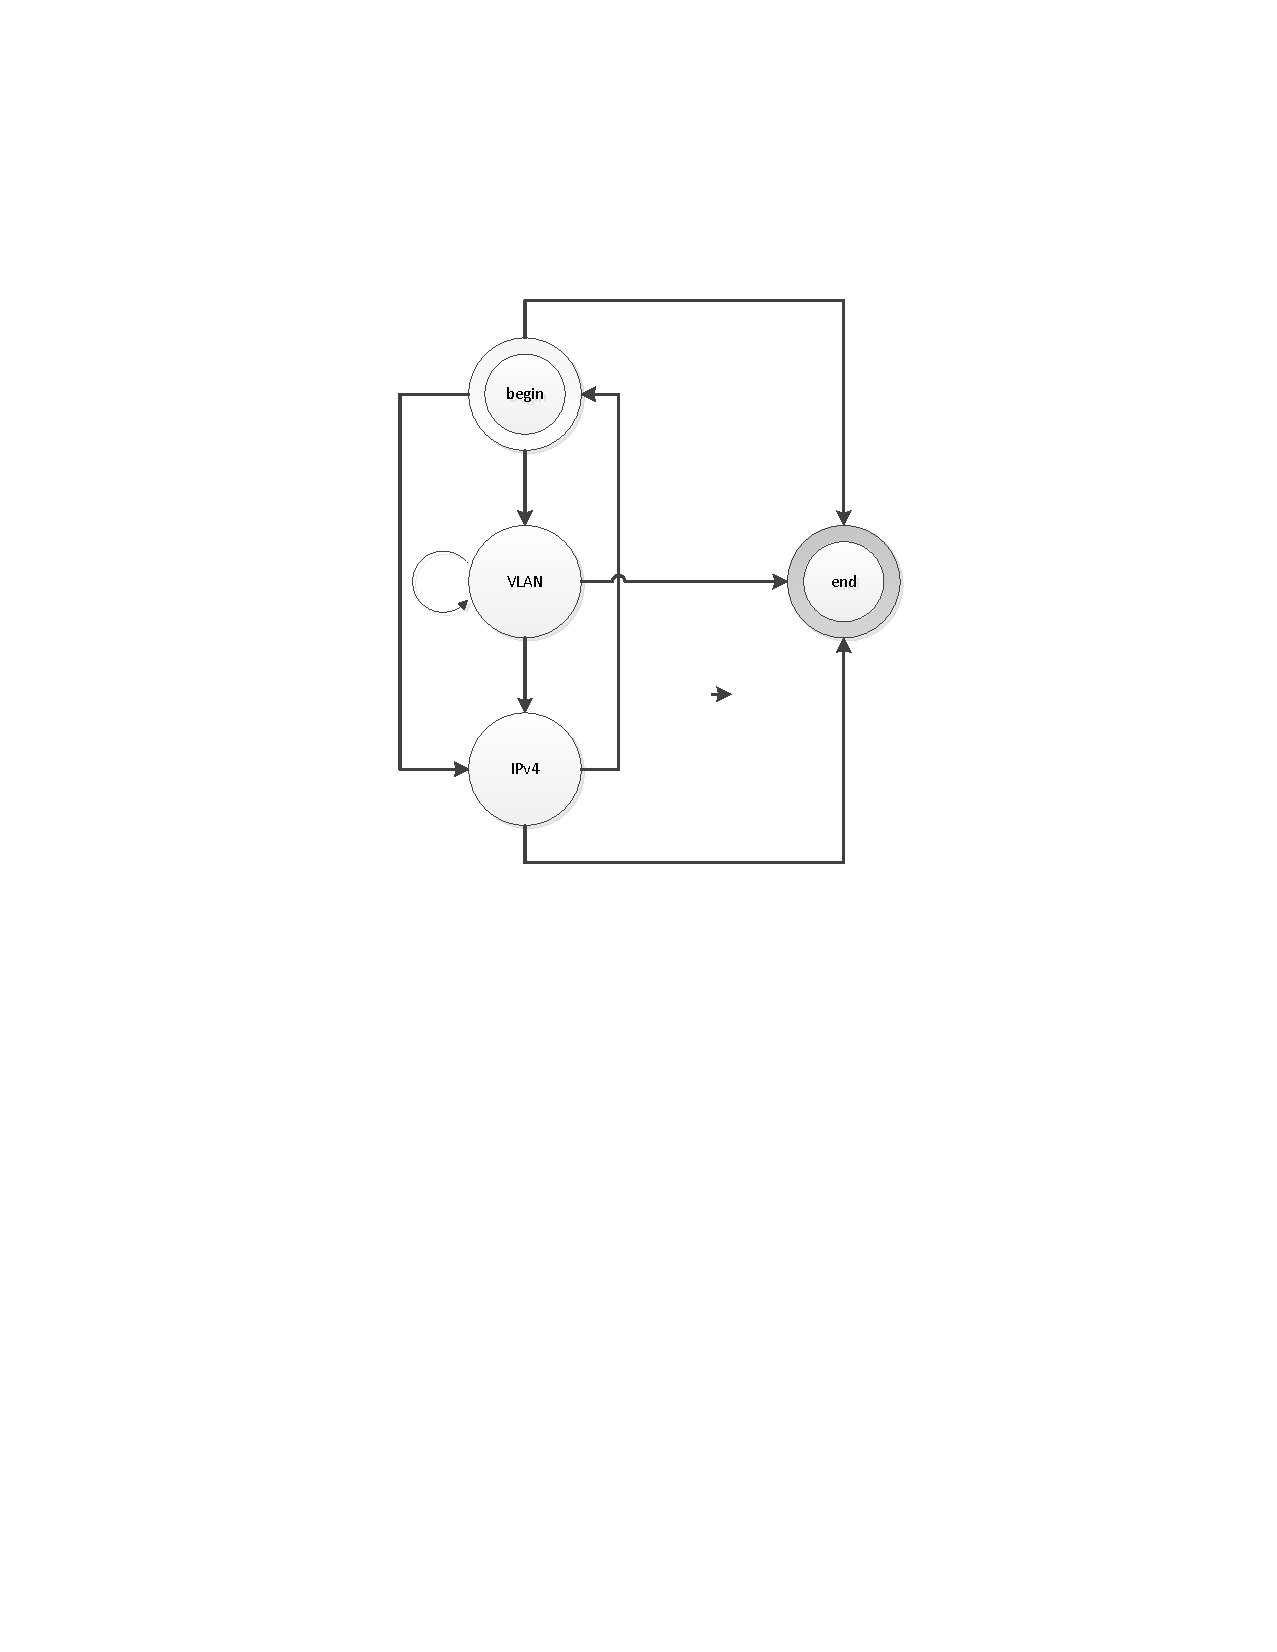
\includegraphics[width=0.7\columnwidth]{image/StateMachine}
	\vspace{-0.15in}
	\caption{Sample State Machine for Header Parser}
	\vspace{-0.15in}
	\label{clicknp:fig:StateMachine}
	%    
\end{figure}

Above code implement a sample header parser in figure \ref{clicknp:fig:StateMachine}, each state is set to repeat at most twice. 44 lines of code with 3 states generates 314 lines of code with 27 states, which takes 2\% logic resource.

Following show some parsers to extract metadata from some well-known protocols. The element code can be easily modified to extract new fields or incorporate new protocols.

\begin{table}[h!]
	\centering
	\label{clicknp:tab:PacketParsers}
	\begin{tabular}{l|r|r|r}
		Element & LOC & Logic & Memory \\
		\hline
		EthVlanParser & & \% & \% \\
		IPv4\_Parser & & \% & \% \\
		IPv6\_Parser & & \% & \% \\
		FlowTuple\_Parser & & \% & \% \\
		TCP\_Parser & & \% & \% \\
		NVGRE\_Parser & & \% & \% \\
		VXLAN\_Parser & & \% & \% \\
	\end{tabular}
\end{table}

\subsection{Lookup Tables}
\label{clicknp:subsec:lookuptables}

\textit{HashTable} is implemented using Cuckoo hash \cite{pagh2004cuckoo} with two memory banks, which can be used for exact matching.

\begin{figure}[h!]
	\centering
	
\includegraphics[width=0.6\columnwidth]{image/logo}
	\vspace{-0.15in}
	\caption{HashTable Collision Rate, x: occupancy, y: hash collision rate, lines: sequential IP, sequential port, random, theory}
	\vspace{-0.15in}
	\label{clicknp:fig:HashTableCollisionRate}
	%    
\end{figure}

\textit{TCAM} compares all entries in parallel and finds the lowest entry index that matches. Due to high logic resource utilization of TCAMs, we design \textit{HashTCAM} to trade off logic with memory. The design bases on an observation that bit-mask patterns in a set of real-world wildcard rules are limited. In order to reduce bit width of match key, commodity switching chips require users to specify bit-mask patterns prior to rule insertion, e.g. Broadcom Trident II \cite{broadcomethernet} only supports 16 bit-mask patterns.

HashTCAM also imposes a limitation on number of bit-mask patterns. For each unique bit-mask pattern, HashTCAM allocates a HashTable and fills its mask field. All rules sharing this bit-mask pattern can be inserted into HashTable whose key is masked original key and value is the index in original TCAM. Match results from HashTables are arbitrated to find the lowest index (highest priority) and get match result by index from SRAM. The \textit{HashTCAM} class in host program provides TCAM-like interface to abstract away HashTable allocation, rule update and SRAM update.

\begin{figure}[h!]
	\centering
	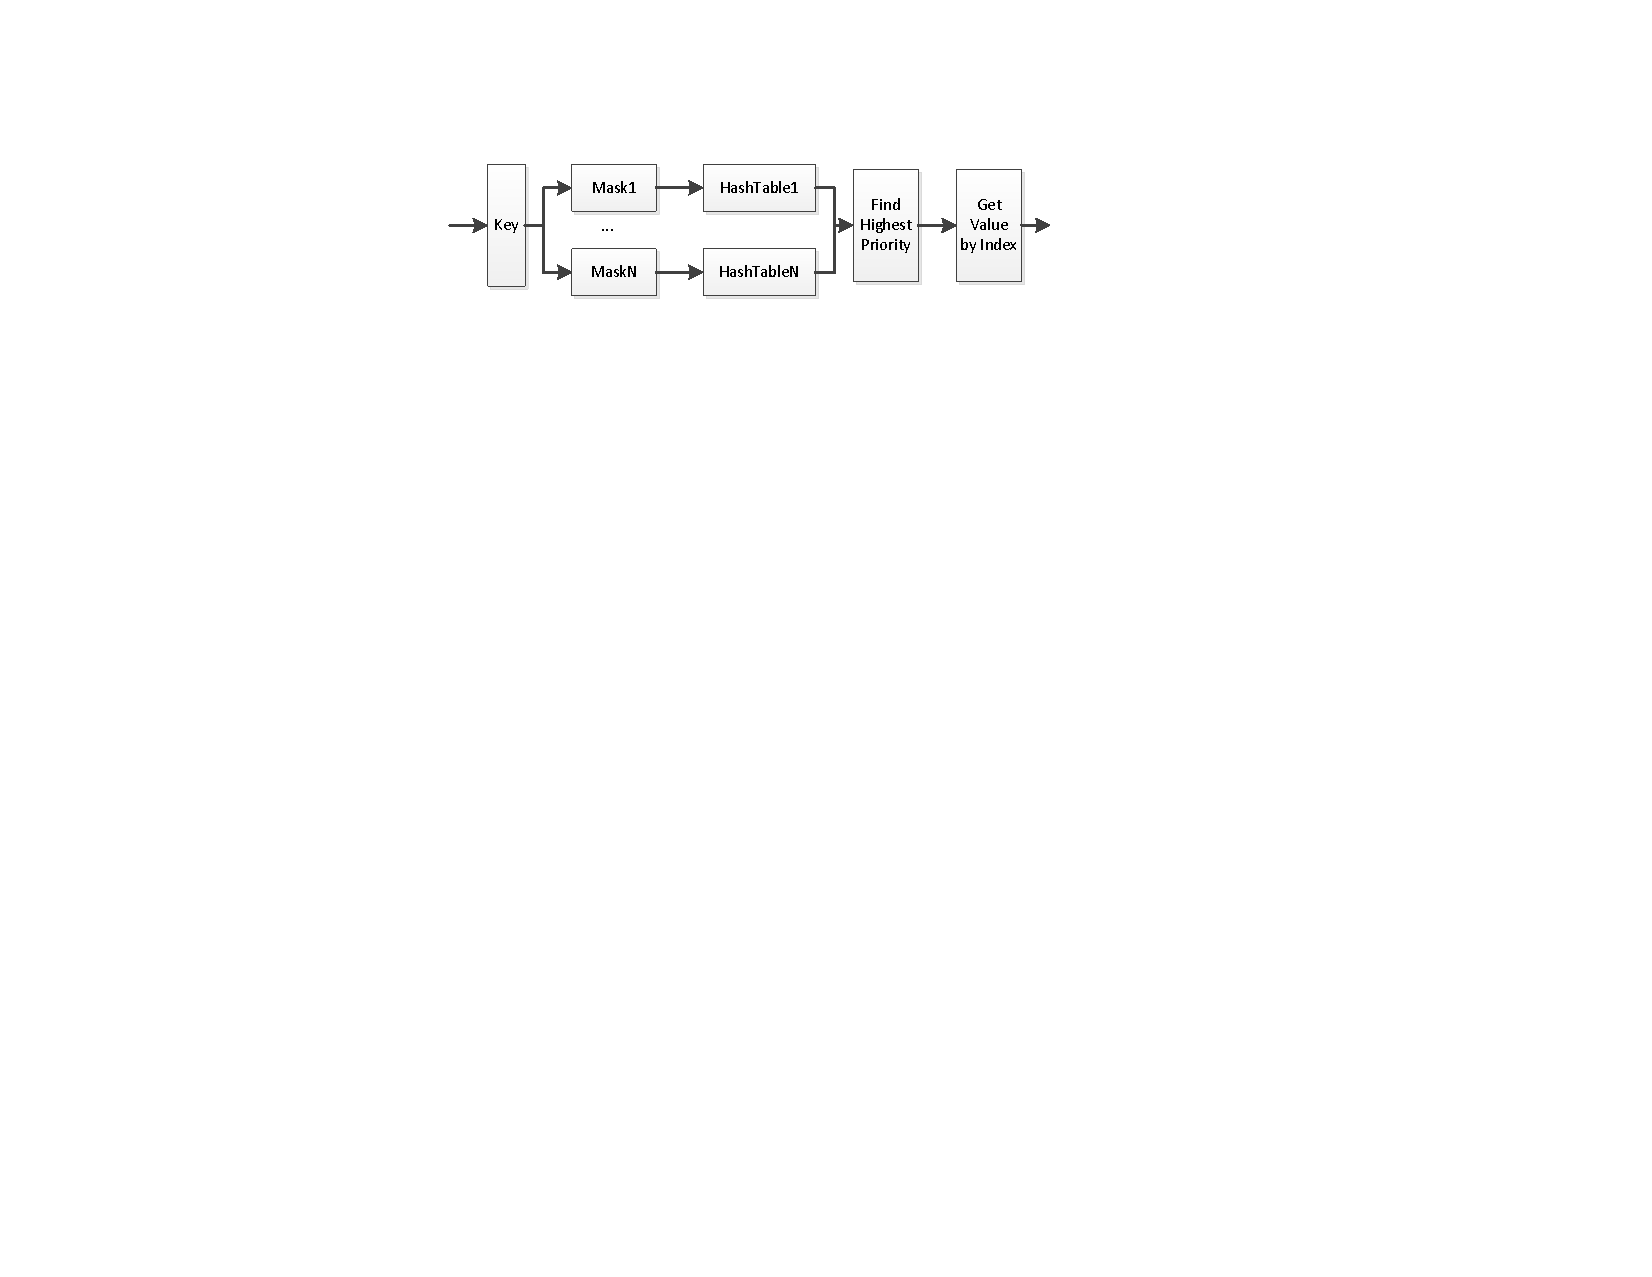
\includegraphics[width=1.0\columnwidth]{image/HashTCAM}
	\vspace{-0.30in}
	\caption{HashTCAM Architecture}
	\vspace{-0.10in}
	\label{clicknp:fig:HashTCAM}
	%    
\end{figure}

Longest Prefix Match (\textit{LPM}) is essentially the \textit{IP\_Lookup} example in section \ref{clicknp:subsec:elementdef}.

HashTable, TCAM, HashTCAM and LPM tables all match metadata, while deep packet inspection requires matching packet content. Content matching is much more resource hungry than matching a fixed offset in packet. \textit{StringMatch} works by comparing all offsets of a flit with the pattern byte-by-byte in parallel. \textit{RegexMatch} compiles multiple regexes into one NFA (nondeterministic finite automaton) and build a 32-level pipeline to process next byte and update NFA's active states every stage, similar to the \textit{IP\_Lookup} example. Due to logic resource constraint, current implementation of \textit{RegexMatch} compiles the NFA into FPGA image and does not allow on-the-fly regex reconfiguration.

\begin{table}[h!]
	\centering
	\label{clicknp:tab:LookupTables}
	\begin{tabular}{l|r|r|r|r|r}
		Element & LOC & Key width & Size & Logic & Memory \\
		\hline
		HashTable 	& & 104b & 32K 	& 5\%  & 10\% \\
		TCAM 		& & 104b & 64	& 20\% & 0\% \\
		HashTCAM 	& & 104b & 16K    & 10\% & 10\% \\
		LPM			& & 32b  & 16K    & 10\% & 10\% \\
		StringMatch & & 32B  & 100	& & \\
		RegexMatch  & & 32B  & 100  & & \\
	\end{tabular}
\end{table}

Most signal handlers take only several cycles, so the update rate for lookup tables is bounded by the latency of PCIe channel: 120K updates per second in interrupt mode and 500K updates per second in polling mode.

\subsection{Packet Modifications}

\begin{table}[h!]
	\centering
	\label{clicknp:tab:PacketModElements}
	\begin{tabular}{l|r|r|r}
		Element & LOC & Logic & Memory \\
		\hline
		PacketModifier 	& & \% & 0\% \\
		PushHeader		& & \% & 0\% \\
		PopHeader		& & \% & 0\% \\
		DropPolicer 	& & \% & \% \\
	\end{tabular}
\end{table}

\subsection{Traffic Schedulers}

\begin{table}[h!]
	\centering
	\label{clicknp:tab:TrafficSchedulers}
	\begin{tabular}{l|r|r|r}
		Element & LOC & Logic & Memory \\
		\hline
		GenericPriorityQueue 	& & \% & 0\% \\
		RoundRobin		& & \% & 0\% \\
		WeightRoundRobin		& & \% & 0\% \\
		StrictPriority		& & \% & 0\% \\
		TokenBucket 	& & \% & \% \\
	\end{tabular}
\end{table}
